\chapter{Introduction}
\label{chap:introduction}

Altough high temperature superconductivity has been known for almost three decades \cite{Bednorz1986}, a satisfactory explanation of this phenomenom still remains as one of the major unsolved problems in theoretical condensed matter physics. 
It is known that, similarly to BCS theory \cite{Bardeen1957}, high-temperature superconductivity is caused by attraction between electrons \cite{?}. 
However it remains unclear how this attraction arises, when it is sizable and when it is not, and what factors are detrimental to superconductivity.

In contrast to the BCS theory \cite{Bardeen1957}, the pairing mechanism in the \textit{unconventional superconductors} (cuprates, iron-based and heavy fermion \cite{Pfleiderer2009}) is unknown.
Two leading theories: resonating-valence-bond \cite{?} and spin fluctuation \cite{Scalapino2012} rely heavily on magnetic interactions while mostly ignoring the lattice effects.

Soon after their discovery Anderson proposed \cite{Anderson1987} that the parent compounds are in a \textit{quantum spin liquid} phase that do not break any symmetries. 

In this theory, also called the \textit{resonating valence bond} (RVB), he argues that
\begin{quote}
  The preexisting magnetic singlet pairs of the insulating state become charged superconducting pairs when the insulator is doped sufficiently strongly. 
The mechanism for superconductivity is hence predominantly electronic and magnetic, although weak phonon interactions may favor the state.
\end{quote} 

\cite{Chakravarty2008}: Breaking of RVB

The high-T$_c$ cuprate superconductors have complex phase diagrams with many competing ground states and quantum phase transitions between them \cite{Chakravarty2011}.
Parent compounds of copper based superconductors start out as insulators and become superconductors when doped with additional charge carriers.
Depending on the compound, superconducting charge carriers can be either electrons or holes.
We show a simplified phase diagram for several cuprate superconductors in Figure \ref{fig:CuPhaseDiag} which highlights some of common characteristics between them.
For low charge carriers concentration the parent compounds form ordered crystalline structures and exhibit antiferromagnetism below a certain temperature $T_N$ \cite{?}.
This antiferromagnetic phase is suppresed by charge doping giving rise to superconductivity.
Antiferromagnetism and superconductivity seem to be excluyent \cite{?}, however they appear in close proximity in the phase diagram.
After the antiferromagnetism is suppressed, the superconducting transition temperature (T$_c$) rises with doping until it reaches a maximum value for some optimal doping level finally decreasing to zero for greater dopings.

\begin{figure}[ht]
  \centering
  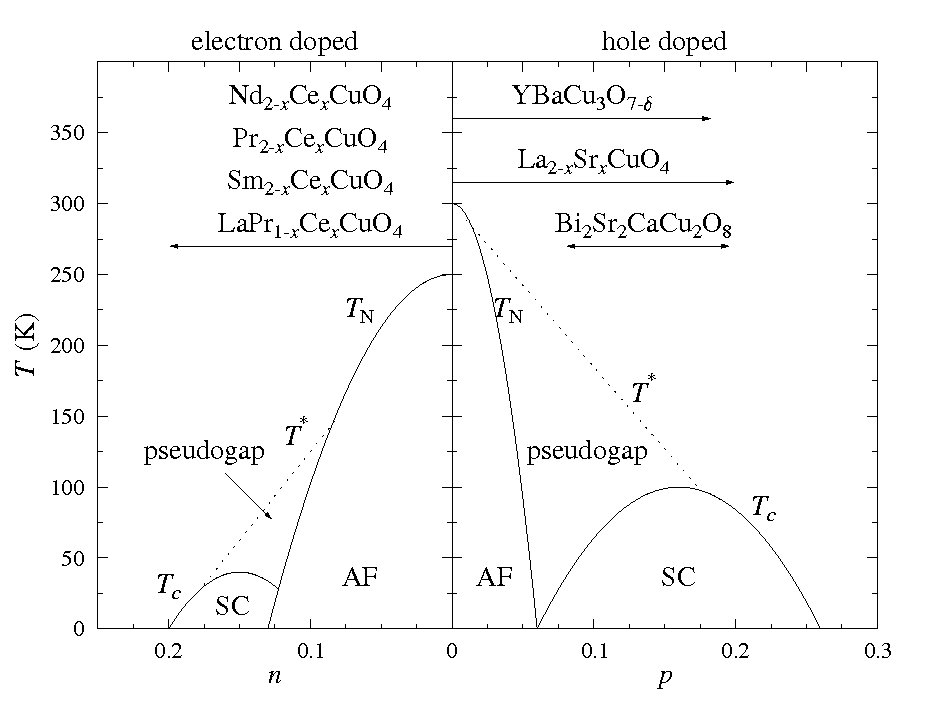
\includegraphics[width=0.8\textwidth]{images/CuPhaseDiag.png}
  \caption[Simplified version of the cuprate superconductor phase diagram]
  {Simplified version of the cuprate superconductor phase diagram \protect\cite{CuPhaseDiag}.}
  \label{fig:CuPhaseDiag}
\end{figure}

One defining property of a superconductor, within the band energy approximation, is the presence of an energy gap, but early experiments could not find its characteristic signatures in cuprate superconductors.
Instead of abruptly finding a zero density of states below a certain energy at the superconducting transition temperature there was only a partial depression of excitations appearing at a much higher temperature T*.
This region of phase space has been identified as the \textit{pseudogap phase} and there is evidence for its presence in all cuprate superconductor families \cite{Timusk1999,Muller2007}.
This phase seems to precede superconductivity for a large part of the phase diagram but its relationship to superconductivity still remains unclear \cite{?}.

In addition to the partial gap, the pseudogap phase presents many interesting characteristics. 
One of them is the observation of lattice inhomogeneities breaking the crystalline translational symmetry.
For example in La$_{1.85}$Sr$_{0.15}$CuO$_{4}$ and La$_{2}$CuO$_{4.1}$, the dopant atoms, necessary for superconductivity, do not reside at the crystal symmetric sites making these compounds structurally inhomogeneous \cite{Poccia2011}.
In YBa$_2$Cu$_3$O$_{7-\delta}$ (YBCO) the dopant atoms reside in crystal symmetric positions but the departure from stoichiometry produces compositional disorder \cite{Chen1988,Andersen1990} making YBCO also an inhomogeneous system.
Even though the dopant atoms are at fixed positions, these structural inhomogeneities have a dynamical character \cite{Mihailovic2005,Bianconi1996}.
Such a dynamical inhomogeneity is present even in some compounds with perfect crystallographic symmetry like HoBa$_{2}$Cu$_{4}$O$_{8}$ \cite{RubioTemprano2000}.
Although from the structural inhomogeneity does not necessarily follow an inhomogeneous electronic ground state, for some regions of the phase diagram, depending on the dopant concentation, such state is realized \cite{?}.

In addition to the breaking of the crystalline translational symmetry the pseudogap phase exhibits other broken symmetries. 
Time-reversal symmetry breaking was found using angular resolved photoemission spectroscopy with circularly polarized photons in Bi$_{2}$Sr$_{2}$CaCu$_{2}$O$_{8+\delta}$ \cite{Kaminski2002}. 
The crystalline rotational symmetry is broken locally in La$_{1.85}$Sr$_{0.15}$CuO$_{4}$ with alternating regions of tetragonal and orthorhombic symmetry \cite{Bianconi1996} according to x-ray absorption spectroscopy. 

The clues provided by these broken symmetries should yield an understanding of the ground state in this pseudogap phase, its elementary excitations and the appearance of superconductivity at temperatures below the onset of the pseudogap. 

% Polaronic nature of the carriers
Carriers are polaronic objects \cite{Zhao1997}
\begin{quote}
  Here we report the results of magnetization and thermal expansion measurements on samples of the copper oxide superconductor La$_{2-x}$Sr$_x$CuO$_4$ which characterizes the oxygen-isotope effect on the carrier density and on the in-plane penetration depth. We find a neglible isotope effect on the former, but a large on the latter. Specific quantitative features of the results show that polaronic charge carriers exist and condense into Cooper pairs in the copper oxide superconductors.
\end{quote}

\cite{Kresin2009}: ``Electron-lattice interaction and its impact in high-T$_c$ superconductivity'' 
This charge-lattice dynamic is inacessible within the Born-Oppenheimer approximation, thus an exact treatment is necessary.
We focus on a small but important subsytem and study a model hamiltonian for it that explains some of the experimental evidence

The remainder of this introductory chapter is devoted to reviewing some of the experimental results pointing to the importance of considering the lattice and electronic inhomogeneities in the description of superconductivity. 
We start, in section \ref{sec:dynamicDistortions} with an overview of the dynamic local lattice distortions in cuprates incluiding the important feature of stripes. 
Afterwards, in section \ref{sec:electronic_inhomogeneity}, we turn our attention to electronic inhomogeneities. 
In sections \ref{sec:phonon_spectra} and \ref{sec:specific_heat} we present some experimental anomalies in the phonon spectra and specific heat respectively and speculate about their possible origin in the mentioned inhomogeneities. 
Next we duscuss some of the controversial experimental results in isotopic effects and ultrafast spectroscopy in sections \ref{sec:isotopic_effects} and \ref{sec:ultrafast_spect} respectively.

In the last part of this introduction we limit the scope of this thesis and present our motivation and approach at describing these dynamic effects (sec. \ref{sec:scope}) and provide an outline of the next chapters.


\section{Dynamic local lattice distortions}
\label{sec:dynamicDistortions}

All cuprate high-T$_c$ superconductors consist of a given number $n$ of CuO$_2$ planes separated by \textit{charge reservoirs}.
Some materials, such as La$_{2-x}$Sr$_x$CuO$_4$ and Nd$_{2-x}$Sr$_x$CuO$_4$, have one CuO$_2$ plane per unit cell. 
Other compounds like Bi$_2$Sr$_2$Ca$_{n-1}$Cu$_n$O$_{2n+4+x}$ have been synthesized with $n=1,2$ and 3 CuO$_2$ planes \cite{Basov2005}.
In this thesis we give particular attention to YBa$_2$Cu$_3$O$_{7-\delta}$ (YBCO) which has two CuO$_2$ layers and is one of the most commonly studied compounds.

The crystal structure of YBa$_2$Cu$_3$O$_6$ ($\delta=1$) is tretragonal (\textit{P4/mmm} space group) whereas YBa$_2$Cu$_3$O$_7$ ($\delta=0$) is orthorrombic (\textit{Pmmm} space group).
The oxygen atoms in YBCO occupy four inequivalent positions and are usually labelled as follows: O(1) is in the Cu-0 \textit{chains}, O(2),O(3) are in the Cu-0 \textit{planes}, and O(4) is the \textit{apical} oxygen (see Figure \ref{fig:YBCO_structure}).
Each oxygen contributes in a different way to the several properties of the material.
The sites O(2), O(3), and O(4) are always filled whereas, depending on the value of $\delta$, the population of the O(1) sites varies.
The $\delta$ value depends on the growing and treatment conditions specially on the thermal annealing at different atmospheres or vacuum \cite{Ivanov1995}.
The two copper atoms in the unit cell also occupy two inequivalent positions.
The labels Cu(1) and Cu(2) are usually assigned to copper atoms in the chains and CuO$_2$ planes respectively.
It is commonly accepted that the Cu(1)-O(1) chains serve as reservoirs for excess holes \cite{Pickett1989}. 
At low $\delta$ the holes are localized at the chains and do not contribute to the conductivity at low temperatures however,
at larger $\delta$ a hole transfer occurs to the Cu(2)-O(2),O(3) planes and the samples become superconducting \cite{Cava1988}.

\begin{figure}[ht]
  \centering
  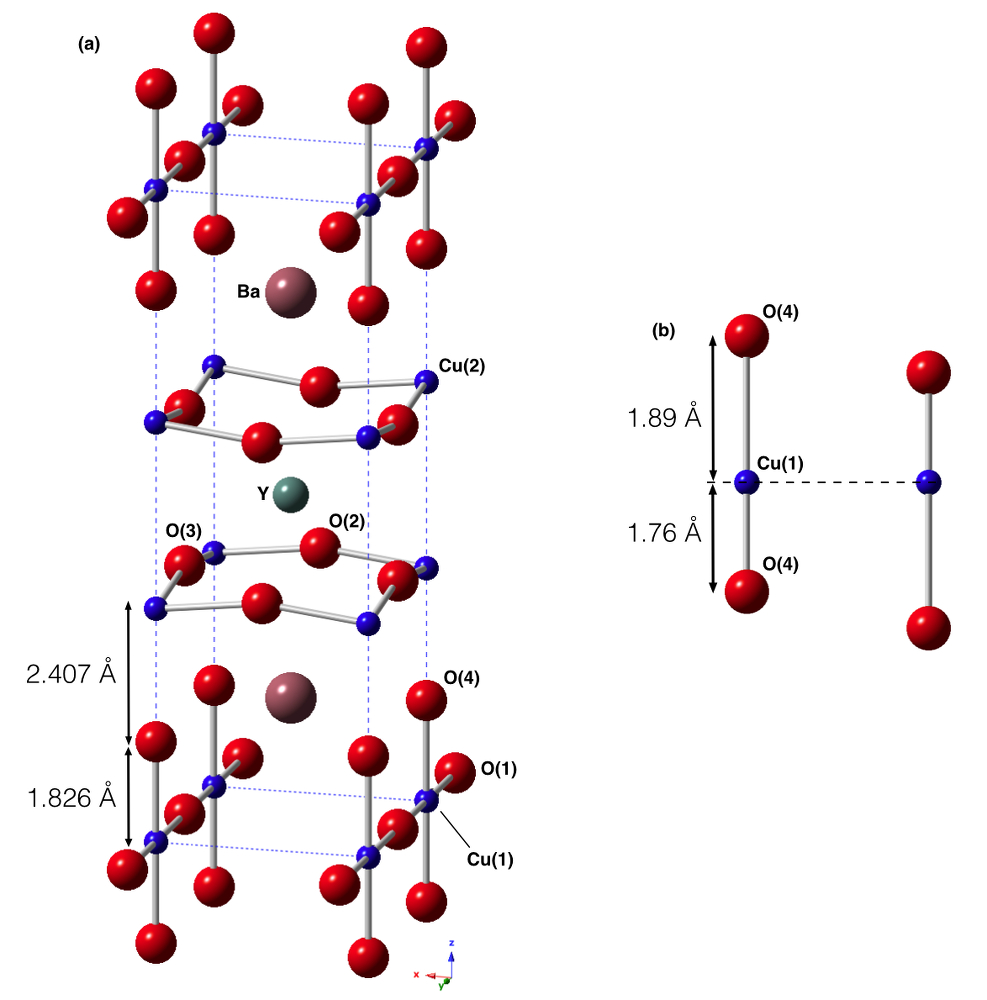
\includegraphics[width=0.7\textwidth]{images/YBCO_O-Cu-O.jpg}
  \caption[Crystal structure of YBa$_{2}$Cu$_{3}$O$_{7}$ and the two possible O(4)-Cu(1)-O(4) configurations.]
  {\textbf{(a)} Crystal structure of YBa$_{2}$Cu$_{3}$O$_{7}$. The dashed line denotes de unit cell. \textbf{(b)} The two possible configurations in the O(4)-Cu(1)-O(4) cluster due to the split O-Cu bond distances (not to scale).}
\label{fig:YBCO_structure}
\end{figure}

Crystal structure in cuprates was determined first by diffraction methods without any sign of significant distortions associated with the in-plane nor with the apical oxygen atoms \cite{Capponi1987,Schafer1988}. 
One of the first observations of a local lattice distortion in cuprates was made using Cu K-edge extended X-ray absorption fine structure (EXAFS) measurements.
It showed a two distances for the Cu(1)-O(4) bond length in YBa$_2$Cu$_3$O$_7$ at temperatures above the superconducting transition temperature, T$_{c}$, with a difference in length close to 0.13 \AA\ \cite{MustredeLeon1990,Conradson1990}.
Since the average bond lengths in diffraction has a significantly higher precision ($\sim 0.001$ \AA \cite{Miceli1988}) than local probes like EXAFS \cite{Rehr2000}, these reports were controversial \cite{Kwei1990}.
To resolve the controversy, it was noticed that the time scale in EXAFS measurements is such that dynamical distortions can be measured but, depending on the size of the distortion, elastic techniques like X-ray or neutron diffraction are unable to detect them \cite{Salkola1995}.
For example, it was shown that the two-site O(4) distribution in in Tl$_{2}$Ba$_{2}$CaCu$_{2}$O$_{8}$ could be only detected in a pair distribution function obtained from neutron inelastic scattering but not with that obtained from neutron diffraction \cite{Egami1991}. 
Consequently, it is important to take into account both the spatial resolution and time resolution of the techniques used to study the actual atomic structure of these materials \cite{Mihailovic2005}. 
The explanation of the discrepancies between these results with diffraction and optical spectroscopical results lead to the interpretation of this two-sites Cu(1)-O(4) distribution as a dynamical distortion of polaronic origin \cite{MustredeLeon1992}.

The EXAFS analysis showed two different Cu(1)-O(4) distances in YBa$_2$Cu$_3$O$_7$ differing by $\sim 0.10-0.13$ \AA \cite{Conradson1990,MustredeLeon1992a} that changed into a single site distribution in the vicinity of the superconducting transition temperature. 
These measurements were carried out using polarized x-rays on magnetically oriented powders, an improvement in the technique which allowed to isolate the Cu(1)-O(4) signal with an increased sensitivity not achievable for the Cu-O EXAFS signal in other cuprates. 
This result was received with skepticism, based on earlier diffraction results \cite{battlog1992lattice,Kwei1990,Sharma1991} and optical spectroscopy \cite{Thomsen1993}. 
Independent EXAFS measurements in other oriented samples \cite{Stern1993} and single crystals \cite{Booth1996} also showed a two-site distribution in YBa$_{2}$Cu$_{3}$O$_{6.7}$, YBa$_{2}$Cu$_{3}$O$_{6.5}$ and Co doped  YBa$_2$Cu$_{2.8}$Co$_{0.2}$O$_{7+\delta}$ \cite{MustredeLeon1991}. 

Similar two site distributions obtained from EXAFS spectra were found for the Cu(2)-O(4) distribution in Bi$_{2}$Sr$_{2}$CaCu$_{2}$O$_{8}$ \cite{bianconni1992lattice} and in TlBa$_{2}$Ca$_{3}$Cu$_{4}$O$_{11}$ \cite{Allen1991} starting at temperatures above T$_{c}$. 
In these compounds (and other cuprates) the average Cu(2)-O(4) bond length lies between 2.49 and 2.73 \AA, which is much longer than the Cu(1)-O(4) bond length in YBa$_{2}$Cu$_{3}$O$_{7}$ ($\sim 1.87$ \AA). 
This fact makes more difficult the identification of details of the O(4) distribution due to the stronger mixing of the Cu(2)-O(4) EXAFS signal with those of other atoms and the increased zero point motion of the O(4) atom due to weaker Cu(2)-O(4) bond compared with the Cu(1)-O(4) bond.
For this reason in most EXAFS studies addressing the O(4) motion a gaussian single site broadened distribution has been used, reporting only changes in the width of the distribution as a function of temperature \cite{Booth1995,Oyanagi2007,Zhang2009}.

In plane Cu(2)-O local lattice distortions were identified in La$_{1.85}$Sr$_{0.15}$CuO$_{4}$ appearing below 100 K \cite{Bianconi1996,Oyanagi2007}, in TIBa$_{2}$CuO$_{6}$ below 120 K \cite{Conradson1997} and in La$_{2}$CuO$_{4.1}$ below 150 K \cite{Lanzara1997,MustredeLeon:xj5003}. 
In this case the observation of such distortions in YBa$_{2}$Cu$_{3}$O$_{7}$ and related compounds becomes more difficult due the similarity in Cu-O bond lengths in the CuO$_2$ planes and chains, whose contributions are mixed in the EXAFS signal \cite{Conradson1997,MustredeLeon1992a}.

Until now only in La$_{1.85}$Sr$_{0.15}$CuO$_{4}$ has been possible to identify local lattice distortions involving both in plane oxygen and apical oxygen atoms  \cite{Bianconi1996}. 
We also stress that from all these EXAFS experiments it is only possible to probe with enough detail the nearest neighbor environment around the Cu atoms, thus the spatial extension of the distortions cannot be determined solely from these measurements. 
Additional structural information \cite{Bianconi1996a} is needed to formulate models about the extension of the distortions as discussed in Ref. \cite{Bianconi1996}.

Pair distribution function analysis of diffraction, X-ray and neutron inelastic scattering can additionally provide information about the intermediate range (up to 10-15 \AA) atomic structure, complementary to the information obtained from EXAFS \cite{Egami2003}. 
Pair distribution function results in La$_{1-x}$Sr$_{x}$CuO$_{4}$ \cite{Bozin1999,Bozin2000} indicate that the atomic structure in this material is a combination of nanoscale regions with different local Cu-O environments, in agreement with the model proposed in Ref. \cite{Bianconi1996}. 
A homogeneous structure only appears when dopant concentrations are above $x = 0.25$. 
In this region the electronic behavior can be described in terms of free fermion quasiparticles.

%Stripes review: \cite{Kivelson2003}
%Very nice review about electrodynamics in High-Tc superconductors: \cite{Basov2005} 

\section{Electronic inhomogeneity}
\label{sec:electronic_inhomogeneity}

STM observations of electronic inhomogeneity in Bi$_2$Sr$_2$CaCu$_2$O$_{8+\delta}$ \cite{Pan2001} \begin{quote}The inhomogeneity is manifested as spatial variations in both the local density of states spectrum and the superconducting energy gap. These variations are correlated spatially and vary on the surprisingly short length scale of approximately 14 \AA. \end{quote}

NMR shows charge density variations (stripes) in YBa$_2$Cu$_3$O$_{7-\delta}$ \cite{Haase2003}

See introduction of this article: \cite{Ivanov1995}

ARPES review: \cite{Damascelli2003}

Raman spectra says: pseudogap is s-wave; superconducting gap is d-wave \cite{Sakai2013}.
Pseudogap is not incipient superconductivity but another kind of order \cite{He2011}

\section{Phonon spectra}
\label{sec:phonon_spectra}

Forbidden ir modes only present below T* \cite{?}

Anomalous ir conductivity in the pseudogap phase \cite{Basov1996}

``Phonon contributions to the specific heat as a function of Co content correlate closely with observed anomalies in calorimetric measurements, indicating that phonons contribute intrinsically to the transition mechanism, e.g. via Bose condensation of structural bipolarons.'' \cite{Obhi1990} 



\section{Electric resistivity}
\label{sec:resistivity}

T vs T$^2$. See v.g. \cite{Timusk1999}

For a Fermi liquid the dc resistance varies as T$^2$.

\cite{Muller2007}: \textit{At optimum doping, i.e- T$_c$ maximum, and in the normal state, the resistivity increases linearly with temperature}

\section{Specific heat}
\label{sec:specific_heat}

Specific heat: \cite{Loram1993}

For a Fermi liquid the specific heat rises linearly with the temperature.

\section{Isotopic effects}
\label{sec:isotopic_effects}

It is possible to make a site-selective substitution $^{16}$O $\rightarrow$ $^{18}$O in YBCO \cite{Conder1993} allowing a precise study of the isotopic effects. 
This has effects in both the phonon frequencies \cite{Ruani1994} and T$_{c}$ \cite{Zech1994,Cardona1988}. 
The \textit{harmonic} approximation accounts well for the O(2)/O(3) vibrations but it fails for O(4) (see again \cite{Ruani1994})

Noticeable isotopic shifts have been used to identify particular excitations as \textit{phononic} in origin (v.g. \cite{Thomsen1990}) however, we will argue, the converse is not true. 
That is, there can be \textit{phononic} excitations without a measurable isotopic shift.

From the isotope effects in the London penetration length follows that the carriers are polaronic objects \cite{Zhao1997}.

From \cite{Khasanov2004} \begin{quote}A substantial isotope shift $\Delta\lambda_{ab}/\lambda_{ab}=2.8(1.0)$\% at 4 K is observed, implying that the in-plane effective supercarrier mass $m^*_{ab}$ is oxygen-isotope dependent with $\Delta m^*_{ab} / m^*_{ab}=5.5(2.0)$\%.\end{quote}

Isotope dependence of the electronic energy bands \cite{Gweon2004}

(small) isotope effects on T$_c$ mainly come from in-plane oxygens \cite{Zech1994}

There's no isotope effect on Tc for 16O$\rightarrow$18O in YBCO \cite{Thomsen1988}

\section{Ultrafast spectroscopy}
\label{sec:ultrafast_spect}

\cite{Smallwood2012}: Using femtosecond lasers they study Cooper-pair recombinations in Bi$_2$Sr$_2$CaCu$_2$O$_{8+\delta}$
\begin{quote}Gap and quasiparticle population dynamics revealed marked dependencies on both excitation density and crystal momentum. Close to the d-wave nodes, the superconducting gap was sensitive to the pump intensity, and Cooper pairs recombined slowly. Far from the nodes, pumping affected the gap only weakly, and recombination processes were faster. These results demonstrate a new window into the dynamical processes that govern quasiparticle recombination and gap formation in cuprates.\end{quote}

\section{Scope and outline of this thesis}
\label{sec:scope}

% Lattice inhomogeneities limit the applicability of $k$-space formalism.
% Correlated electron-lattice motion prevents the use of Born-Openheimer approximation

% A Peierls-Hubbard model has been used there to explain the lattice distortion in terms of bipolarons.
% We explore many other excitations in that model trying to reconcile its predictions with the experimental observations.
% Particular emphasis is given to the isotopic effects because there is controversy around them and they probe the electron-lattice relationship.
% We suggest a possible two-component superconductivity model involving bosonic bi-polaronic objects and free fermions. 
% Chapter outline.

Quantum solid-state theory usually assumes a periodic potential however, since these materials are intrinsically inhomogeneous, it is possible that a successful model needs to abandon such assumption. 
This calls into question the applicability of models based on the \textit{reciprocal space} formalism.
Furthermore, some of the experimental results reviewed in the previous secions suggest that the polaronic behaviour must be taken into account.
This correlated electron-lattice movement prevents the use of the Born-Oppenheimer approximation, which splits the system's wavefunction in electronic and lattice factors $\Psi = \psi_{electronic}\psi_{lattice}$.
Some systems with an important electron-lattice interaction can be treated with perturbation theory either assuming a small (adiabatic) or strong (anti-adiabatic) interaction \cite{?}. 
However, it seems that the electron-lattice interaction in the CuO planes for cuprate superconductors falls in the middle of such extremes \cite{MustredeLeon1992} preventing the use of any such approximation.

We are prompted, therefore, to use an exact model free from the approximations described above. 
The computational complexity of exact models forces us to restrict the system under study to a small subset of the whole compound.
In this work we return to a model describing the peculiar polaronic behaviour of the O(4)-Cu(1)-O(4) cluster in YBa$_{2}$Cu$_{3}$O$_{7}$ approximating the cluster as a system with three sites and two holes \cite{MustredeLeon1992}.
Such approximation is justified as the Cu(1)-O(4) bond length (1.83 \AA) is far shorter than the Cu(2)-O(4) bond length ($\sim$ 2.41 \AA) (see Fig. \ref{fig:YBCO_structure}), making charge transfer outside the cluster a much slower process than the charge dynamics inside the cluster. 
This model provides a very simple framework to explore the charge dynamics influenced by the lattice vibrations and has successfully described the split O(4)-Cu(1)-O(4) distance observed by EXAFS experiments (see section \ref{sec:dynamicDistortions} above).
Although we cannot directly identify the three site cluster proposed in this model with a particular structure of the CuO plane, the general approach of charge transfer between hole rich regions and hole poor regions in the plane coupled to the lattice degrees of freedom is still valid, hence the general conclusions we draw from this model applicable to describe the structure of the CuO plane.

It has been found that superconductivity occurs in the Cu(2)-O(2,3) planes rather than the Cu(1)-O(1,4) chains partially addressed by the model under study in this work.
This raises a question about the relevance of the polaronic behaviour, es explored with this model, to superconductivity.
It is indeed beyond the capability of such a simple model to address the nature of high-temperature superconductiity.
However, it is possible that the polaronic objects in the Cu(1)-O(1,4) chains are capable of providing a pairing mechanism for the Cooper pairs in the Cu(2)-O(2,3) planes.
This will point to a \textit{two component superconductivity} theory similar to some current proposals \cite{?}

% Thesis outline here